\chapter{IMPLEMENTATION AND TESTING}
\section{Implementation}
"Code Connect" is a delightful online space where programmers come together to share ideas and experiences. Using tools like HTML, CSS, and JavaScript, we've built a website that's easy to use and fun to explore. Behind the scenes, PHP and MySQL work like magic to handle all the information. With AJAX and JQuery, everything feels smooth and interactive, just like chatting with friends. It's not just about technology – it's about people connecting and learning from each other. Just like baking a tasty treat, we've mixed all these ingredients to create something special that everyone can enjoy.


% (20\% of Report Length)

% a. Showcase the output at various intermediate stages of the project pipeline

% b. Use proper data visualizing techniques to present the output

% c. Figures and tables must be accompanied by an explanation
\section{Tools Used}
\subsection{Git}
Git is a fundamental version control system for software development, efficiently managing changes through commits. It fosters collaboration via branches and seamless merging, acts as a backup mechanism, and encourages code reviews for quality improvement. Git's popularity in open-source projects facilitates global collaboration, and its integration with CI/CD pipelines automates testing and deployment. In essence, Git empowers teams with version control, collaboration capabilities, and streamlined change management, enhancing project development.
\subsection{Figma}
Figma, a cloud-based design and prototyping tool, is renowned for its real-time collaboration, allowing multiple users to work together seamlessly. It offers robust design features like vector editing, typography controls, and color management. Designers can create interactive prototypes with clickable elements and animations, simulating user interactions effectively. Figma promotes design consistency through component libraries and simplifies handoff with easy sharing of specs and assets. It enhances stakeholder engagement, supports user testing, and integrates with various tools, making it a versatile choice for teams focused on delivering compelling digital experiences.
\subsection{GitHub}
GitHub is a pivotal web-based platform for software development, utilizing Git for version control and centralized code hosting. Multiple developers collaborate simultaneously using branches and pull requests for code review. It boasts an integrated issue tracker, wikis, and documentation for enhanced accessibility. GitHub seamlessly integrates with CI/CD tools and fosters open-source community participation. Security measures include vulnerability scanning and permissions management. In summary, GitHub serves as a collaborative hub for version control, code management, issue tracking, and community involvement, enabling efficient software development.
\subsection{HTML, CSS and JS}
\begin{itemize}
    \item \textbf{HTML (Hypertext Markup Language)}: HTML is the foundational language used to create the structure of web content. It uses a system of tags to define elements like headings, paragraphs, links, images, and more. These tags give structure to web pages, organizing content into a meaningful layout. HTML provides the framework for displaying information and forming the basis for user interaction on the web.

    \item \textbf{CSS (Cascading Style Sheets)}: CSS is a styling language that complements HTML by controlling the visual presentation of web content. It allows developers to define colors, fonts, margins, borders, and other design aspects of HTML elements. By separating content from presentation, CSS enables consistent styling across web pages and enhances user experience through improved aesthetics and readability.

    \item \textbf{JavaScript (JS)}: JavaScript is a versatile scripting language used to add interactivity and dynamic behavior to web pages. It enables developers to create responsive features such as form validation, animations, pop-ups, and real-time updates. JS executes directly in the browser, allowing users to interact with web content without requiring page reloads. It's a crucial component for creating engaging and interactive web experiences.

\end{itemize}
\subsection{MySQL}
MySQL, an open-source relational database management system (RDBMS), excels in organizing structured data for various applications. It's proficient in SQL (Structured Query Language), allowing effortless database creation, data relationships, and advanced queries. MySQL ensures data integrity, speedy retrieval through indexing, and reliable transaction management. It supports collaborative data work with security. Whether for small projects or enterprise endeavors, MySQL's adaptability, strong community, and compatibility make it the go-to choice for data management and robust application development.
\subsection{PHP}
In the realm of web development, PHP stands out as a powerful scripting language, capable of creating dynamic and interactive websites. Integrated seamlessly with HTML, PHP empowers websites to process forms, communicate with databases, and deliver content that adapts to user actions. Its open-source nature fosters a collaborative community of developers. For both beginners and experts, PHP is an invaluable tool, enhancing web projects with its functionality and innovation. It serves as a cornerstone in modern web development, essential for crafting standout websites in the digital landscape.
\section{Modules Used}
\subsection{AJAX}
In the dynamic world of web development, AJAX (Asynchronous JavaScript and XML) stands out as a transformative technique. It combines JavaScript and server communication to enable seamless, asynchronous data exchange. Unlike traditional methods, AJAX allows developers to update specific sections of a web page without full page reloads, enhancing user experience. AJAX's compatibility with data formats like XML and JSON enables efficient data transmission, facilitating real-time updates and interactive web applications. This technique elevates user engagement and pushes modern web development into a new era of possibilities.
\subsection{JQuery}
In the realm of web development, jQuery emerges as a transformative force, simplifying complex tasks and enhancing user interaction. This fast, compact JavaScript library streamlines DOM manipulation, making it effortless to select, modify, and animate HTML elements. jQuery's user-friendly syntax and built-in functions mitigate cross-browser compatibility issues, ensuring seamless development across platforms. Its extensive plugin ecosystem adds pre-built functionalities to projects, abstracting complex JavaScript operations into concise commands for cleaner code and faster development. With capabilities in event handling, animations, and AJAX requests, jQuery accelerates the creation of engaging, feature-rich web applications.
\subsection{MySqli Connect}
In the world of web development and database connectivity, the mysqli\_connect function stands as a fundamental tool worth exploring. Within the PHP programming language, it plays a pivotal role in establishing secure links between web applications and MySQL databases. By providing essential parameters like host, username, password, and database name, developers can effortlessly create a communication channel with MySQL servers. This function is crucial for enabling dynamic and interactive web applications, serving as the foundational bridge for data-driven features. mysqli\_connect significantly contributes to the efficiency and responsiveness of modern database-driven web development, making it an essential component.
\subsection{Google Fonts}
In the realm of web design and typography, Google Fonts emerges as a transformative tool. Its extensive collection of meticulously curated fonts offers designers an array of creative possibilities. Beyond aesthetics, Google Fonts prioritizes user experience, promoting accessible and visually appealing text choices. The user-friendly interface and seamless integration make font selection and embedding effortless. Furthermore, it optimizes performance, ensuring that design enhancements don't hinder website speed. My exploration of Google Fonts highlights its value in enhancing both the aesthetics and accessibility of web content significantly.
\subsection{Font Awesome }
In the world of web design and user interface enhancement, Font Awesome stands out as a remarkable tool. Its extensive icon library, spanning diverse categories, simplifies icon integration into web projects. Font Awesome not only adds visual appeal but also enhances functionality. Using CSS classes for seamless icon incorporation and customization options for size, color, and style, it empowers designers for creative expression. Its compatibility with various frameworks and platforms makes it versatile for all developers. Font Awesome significantly elevates user experiences by adding depth and meaning to digital interfaces, making it an essential asset in crafting captivating and user-centric web applications.
\subsection{Bootstrap}
We have used small portion of bootstrap for quick development of profile dashboard. Bootstrap is a widely-used front-end framework that simplifies web development by providing a collection of pre-designed HTML, CSS, and JavaScript components. With its responsive design, ready-made elements, and customization options, Bootstrap enables developers to create mobile-friendly and visually appealing websites and web applications with ease.
% \subsection{Implementation Details of Modules}
% \section{Testing}
% \subsection{Test Cases for Unit Testing}
% \subsection{Test Cases for System Testing}
\section{Testing}
\subsection{Unit Testing}
Unit testing is a software testing technique where individual units or components of a software application are tested in isolation to ensure that they function correctly. These units can be functions, methods, classes, or even small modules. Unit testing aims to verify that each unit performs as expected, providing developers with confidence that their code works as intended and catches bugs early in the development process.
\\
\textbf{Authenication Unit}\\
Here testing different test cases of authentication system in Code Connect is performed as required:\\
\begin{table}[H]
    \caption{Authenication Unit Testing}
        \label{}
    \begin{tabular}{|p{0.3in}|p{1.2in}|p{1.2in}|p{1.2in}|p{1in}|}
        \hline
        Tests & Test Cases & Input & Expected Output & Actual Output \\
        \hline
            1 & Incorrect Password& Email:\url{test@gmail.com} Password:1234& Incorrect Password& Incorrect Password \\
            \hline
            2 & Incorrect Confirm Password in SignUp & Email:\url{test@gmail.com}
            Password:12345679
            Password:12345678 & Enter Same Password & Enter Same Password \\
            \hline
            3 & Correct Credentials In Login & Email:\url{test@gmail.com}
            Password:12345679 & Redirects to homepage & Redirects to homepage \\
            \hline
\end{tabular}
\end{table}

\textbf{Launch Application when user is not logged-in}\\
\begin{table}[H]
    \caption{Launch Application when user is not logged-in Testing}
        \label{}
    \begin{tabular}{|p{0.3in}|p{1.2in}|p{1.2in}|p{1.2in}|p{1in}|}
        \hline
        Tests & Test Cases & Input &Expected Output & Actual Output \\
        \hline
            1 & Launch application& \url{http://localhost/codeconnect/login/}& Log-In page& Log-In page \\
            \hline
\end{tabular}
\end{table}

\textbf{Launch Application when user is already logged-in}\\
\begin{table}[H]
    \caption{Launch Application when user is already logged-in Testing}
        \label{}
    \begin{tabular}{|p{0.3in}|p{1.2in}|p{1.2in}|p{1.2in}|p{1in}|}
        \hline
        Tests & Test Cases & Input &Expected Output & Actual Output \\
        \hline
            1 & Launch application& \url{http://localhost/codeconnect/home/}& CodeConnect Home page& CodeConnect Home page \\
            \hline
\end{tabular}
\end{table}

\textbf{Code Connect Messenger}\\
\begin{table}[H]
    \caption{Code Connect Messenger Testing}
        \label{}
    \begin{tabular}{|p{0.3in}|p{1.2in}|p{1.2in}|p{1.2in}|p{1in}|}
        \hline
        Tests & Test Cases & Input &Expected Output & Actual Output \\
        \hline
            1 & Code Connect Messenger& \url{http://localhost/codeconnect/messenger/}& Code Connect Messenger&  Code Connect Messenger \\
            \hline
\end{tabular}
\end{table}

\textbf{Send Message}\\
\begin{table}[H]
    \caption{Code Connect Send Message to other user Testing}
        \label{}
    \begin{tabular}{|p{0.3in}|p{1.2in}|p{1.2in}|p{1.2in}|p{1in}|}
        \hline
        Tests & Test Cases & Input &Expected Output & Actual Output \\
        \hline
            1 & Send message& click on messenger button and click on other user that is located at the left side to start a conversations& Sends message to that particular user& Sends message to that particular user \\
            \hline
\end{tabular}
\end{table}

\newpage
\textbf{Receive Message}\\
\begin{table}[H]
    \caption{Code Connect Receive Message from other user Testing}
        \label{}
    \begin{tabular}{|p{0.3in}|p{1.2in}|p{1.2in}|p{1.2in}|p{1in}|}
        \hline
        Tests & Test Cases & Input &Expected Output & Actual Output \\
        \hline
            1 & Receive message& click on messenger button and click on other user that is located at the left side to see the conversation& Display the conversation with that particular user& Display the conversation with that particular user\\
            \hline
\end{tabular}
\end{table}

\textbf{Code Connect Search User}\\
\begin{table}[H]
    \caption{Code Connect Search User Testing}
        \label{}
    \begin{tabular}{|p{0.3in}|p{1.2in}|p{1.2in}|p{1.2in}|p{1in}|}
        \hline
        Tests & Test Cases & Input &Expected Output & Actual Output \\
        \hline
            1 & Code Connect Search User& Si& Name of user starting from "Si"& Sirjan Shrestha \\
            \hline
\end{tabular}
\end{table}

\textbf{Code Connect Search Posts}\\
\begin{table}[H]
    \caption{Code Connect Search Posts Testing}
        \label{}
    \begin{tabular}{|p{0.3in}|p{1.2in}|p{1.2in}|p{1.2in}|p{1in}|}
        \hline
        Tests & Test Cases & Input &Expected Output & Actual Output \\
        \hline
            1 & Code Connect Search Posts& python& Posts that have content of python& python posts \\
            \hline
\end{tabular}
\end{table}

\newpage
\textbf{Show posts of friends only}\\
\begin{table}[H]
    \caption{Show posts of friends only Testing}
        \label{}
    \begin{tabular}{|p{0.3in}|p{1.2in}|p{1.2in}|p{1.2in}|p{1in}|}
        \hline
        Tests & Test Cases & Input &Expected Output & Actual Output \\
        \hline
            1 &Show posts of friends only& Click on the Friends Only button located at post section& Shows Posts of Friends only& Shows posts of friends only \\
            \hline
\end{tabular}
\end{table}

\textbf{Show all posts}\\
\begin{table}[H]
    \caption{Show all posts Testing}
        \label{}
    \begin{tabular}{|p{0.3in}|p{1.2in}|p{1.2in}|p{1.2in}|p{1in}|}
        \hline
        Tests & Test Cases & Input &Expected Output & Actual Output \\
        \hline
            1 &Show all posts& Click on the Public button located at post section& Shows Posts of all users& Shows posts of all users \\
            \hline
\end{tabular}
\end{table}

\textbf{Make Posts}\\
\begin{table}[H]
    \caption{Make Posts Testing}
        \label{}
    \begin{tabular}{|p{0.3in}|p{1.2in}|p{1.2in}|p{1.2in}|p{1in}|}
        \hline
        Tests & Test Cases & Input &Expected Output & Actual Output \\
        \hline
            1 & Make posts& Click on post button& Open Post Menu& Opens Posts Menu \\
            \hline
\end{tabular}
\end{table}

\newpage
\textbf{Making Post including content on both Post and Coding section}\\
\begin{table}[H]
    \caption{Making Post including content on both Post and Coding section Testing}
        \label{}
    \begin{tabular}{|p{0.3in}|p{1.2in}|p{1.2in}|p{1.2in}|p{1in}|}
        \hline
        Tests & Test Cases & Input &Expected Output & Actual Output \\
        \hline
            1 & Making Post including content on both Post and Coding section& Post section:coding in C Code section: printf("Hello World");& post including both of the section& made post including both of the section\\
            \hline
\end{tabular}
\end{table}

\textbf{Delete Posts}\\
\begin{table}[H]
    \caption{Delete Posts Testing}
        \label{}
    \begin{tabular}{|p{0.3in}|p{1.2in}|p{1.2in}|p{1.2in}|p{1in}|}
        \hline
        Tests & Test Cases & Input &Expected Output & Actual Output \\
        \hline
            1 & Delete posts&After visiting self profile, Click on delete post button& Deletion of that particular post& Delets the post \\
            \hline
\end{tabular}
\end{table}

\textbf{Geeking on post}\\
\begin{table}[H]
    \caption{Geeking on post Testing}
        \label{}
    \begin{tabular}{|p{0.3in}|p{1.2in}|p{1.2in}|p{1.2in}|p{1in}|}
        \hline
        Tests & Test Cases & Input &Expected Output & Actual Output \\
        \hline
            1 & Geeking on Posts & Press Geek button& count Geek of users on post & counts Geek of users on post \\
            \hline
\end{tabular}
\end{table}

\newpage
\textbf{Un-Geeking on post}\\
\begin{table}[H]
    \caption{Un-Geeking on post Testing}
        \label{}
    \begin{tabular}{|p{0.3in}|p{1.2in}|p{1.2in}|p{1.2in}|p{1in}|}
        \hline
        Tests & Test Cases & Input &Expected Output & Actual Output \\
        \hline
            1 & Un-Geeking on Posts & Press Geek button again & Deletion of geek count of that user &Delets the geek count of that user \\
            \hline
\end{tabular}
\end{table}

\textbf{Commenting on post}\\
\begin{table}[H]
    \caption{Commenting on post Testing}
        \label{}
    \begin{tabular}{|p{0.3in}|p{1.2in}|p{1.2in}|p{1.2in}|p{1in}|}
        \hline
        Tests & Test Cases & Input &Expected Output & Actual Output \\
        \hline
            1 &Commenting on post & Press comment button and write comment & comment of users on that particular post & comment of users on that particular post \\
            \hline
\end{tabular}
\end{table}

\textbf{Deleting Comment on post}\\
\begin{table}[H]
    \caption{Deleting Comment on post Testing}
        \label{}
    \begin{tabular}{|p{0.3in}|p{1.2in}|p{1.2in}|p{1.2in}|p{1in}|}
        \hline
        Tests & Test Cases & Input &Expected Output & Actual Output \\
        \hline
            1 &Deleting Comment on post & Press delete button & Deletion of comment of that user& Delets the comment of that user \\
            \hline
\end{tabular}
\end{table}

\newpage
\textbf{Saving post}\\
\begin{table}[H]
    \caption{Saving post Testing}
        \label{}
    \begin{tabular}{|p{0.3in}|p{1.2in}|p{1.2in}|p{1.2in}|p{1in}|}
        \hline
        Tests & Test Cases & Input &Expected Output & Actual Output \\
        \hline
            1 &Saving post & Press save button located at right side of post & Save the posts & Saves that post \\
            \hline
\end{tabular}
\end{table}

\textbf{Un-Saving post}\\
\begin{table}[H]
    \caption{Un-Saving post Testing}
        \label{}
    \begin{tabular}{|p{0.3in}|p{1.2in}|p{1.2in}|p{1.2in}|p{1in}|}
        \hline
        Tests & Test Cases & Input &Expected Output & Actual Output \\
        \hline
            1 &Un-Saving post & Press save button again that is located at right side of post & Removes the saved post &  Removes the saved post  \\
            \hline
\end{tabular}
\end{table}

\textbf{Profile Dashboard}\\
\begin{table}[H]
    \caption{Profile Dashboard Testing}
        \label{}
    \begin{tabular}{|p{0.3in}|p{1.2in}|p{1.2in}|p{1.2in}|p{1in}|}
        \hline
        Tests & Test Cases & Input &Expected Output & Actual Output \\
        \hline
            1 &Visiting Profile Dashboard & Press on Profile Dashboard button after visiting self-profile &Show the profile Dashboard menu &Opens the profile Dashboard menu  \\
            \hline
\end{tabular}
\end{table}

\newpage
\textbf{Update Basic Account Details}\\
\begin{table}[H]
    \caption{Update Basic Account Details Testing}
        \label{}
    \begin{tabular}{|p{0.3in}|p{1.2in}|p{1.2in}|p{1.2in}|p{1in}|}
        \hline
        Tests & Test Cases & Input &Expected Output & Actual Output \\
        \hline
            1 &Update Basic Account Details & Press on Update Basic Account Details button after visiting profile dashboard &Opens the form that helps the user to update their basic informations  &Opens the form that helps the user to update their basic informations  \\
            \hline
\end{tabular}
\end{table}

\textbf{Update Projects}\\
\begin{table}[H]
    \caption{Update Projects Testing}
        \label{}
    \begin{tabular}{|p{0.3in}|p{1.2in}|p{1.2in}|p{1.2in}|p{1in}|}
        \hline
        Tests & Test Cases & Input &Expected Output & Actual Output \\
        \hline
            1 &Update Projects & Press on Update Projects button after visiting profile dashboard &Opens the form that helps the user to update their Projects  &Opens the form that helps the user to update their Projects  \\
            \hline
\end{tabular}
\end{table}

\textbf{Update Certification}\\
\begin{table}[H]
    \caption{Update Certification Testing}
        \label{}
    \begin{tabular}{|p{0.3in}|p{1.2in}|p{1.2in}|p{1.2in}|p{1in}|}
        \hline
        Tests & Test Cases & Input &Expected Output & Actual Output \\
        \hline
            1 &Update Certification & Press on Update Certification button after visiting profile dashboard &Opens the form that helps the user to update their Certifications  &Opens the form that helps the user to update their Certifications  \\
            \hline
\end{tabular}
\end{table}

\newpage
\textbf{Update Skills}\\
\begin{table}[H]
    \caption{Update Skills Testing}
        \label{}
    \begin{tabular}{|p{0.3in}|p{1.2in}|p{1.2in}|p{1.2in}|p{1in}|}
        \hline
        Tests & Test Cases & Input &Expected Output & Actual Output \\
        \hline
            1 &Update Skills & Press on Update skills button after visiting profile dashboard &Opens the form that helps the user to update their skills  &Opens the form that helps the user to update their skills  \\
            \hline
\end{tabular}
\end{table}

\textbf{Update CV}\\
\begin{table}[H]
    \caption{Update CV Testing}
        \label{}
    \begin{tabular}{|p{0.3in}|p{1.2in}|p{1.2in}|p{1.2in}|p{1in}|}
        \hline
        Tests & Test Cases & Input &Expected Output & Actual Output \\
        \hline
            1 &Update CV & Press on Update CV button after visiting profile dashboard &Opens the form that helps the user to update their CV  &Opens the form that helps the user to update their CV  \\
            \hline
\end{tabular}
\end{table}

\textbf{Code Connect Notification}\\
\begin{table}[H]
    \caption{Code Connect Notification Testing}
        \label{}
    \begin{tabular}{|p{0.3in}|p{1.2in}|p{1.2in}|p{1.2in}|p{1in}|}
        \hline
        Tests & Test Cases & Input &Expected Output & Actual Output \\
        \hline
            1 &Notification & Press on Notifiation button that is located at nav-bar &Open Notification Pannel that shows all the necessary notification &Open Notification Pannel that shows all the necessary notification \\
            \hline
\end{tabular}
\end{table}

\textbf{Send connection request}\\
\begin{table}[H]
    \caption{Send connection request Testing}
        \label{}
    \begin{tabular}{|p{0.3in}|p{1.2in}|p{1.2in}|p{1.2in}|p{1in}|}
        \hline
        Tests & Test Cases & Input &Expected Output & Actual Output \\
        \hline
            1 &Send connection request & After visiting other user's profile, Press on connect button that is located at side bard  &Send connection request to that particular user &Sends connection request to that particular user and shows connection reuested \\
            \hline
\end{tabular}
\end{table}

\textbf{Accept connection request}\\
\begin{table}[H]
    \caption{Accept connection request Testing}
        \label{}
    \begin{tabular}{|p{0.3in}|p{1.2in}|p{1.2in}|p{1.2in}|p{1in}|}
        \hline
        Tests & Test Cases & Input &Expected Output & Actual Output \\
        \hline
            1 &Accept connection request & Click on Accept Request button &Accept connection request of that particular user &Accept connection request of that particular user and adds that user to the connection list \\
            \hline
\end{tabular}
\end{table}

\newpage
\textbf{User Log-Out}\\
\begin{table}[H]
    \caption{User Log-Out Testing}
        \label{}
    \begin{tabular}{|p{0.3in}|p{1.2in}|p{1.2in}|p{1.2in}|p{1in}|}
        \hline
        Tests & Test Cases & Input &Expected Output & Actual Output \\
        \hline
            1 &User Log-Out & Click on Log-Out button that is located at the nav-bar &Logs the user out of the system &Logs the user out of the system and redirect the user to Log-In page \\
            \hline
\end{tabular}
\end{table}
% \begin{figure}[ht]
%     \centering
%     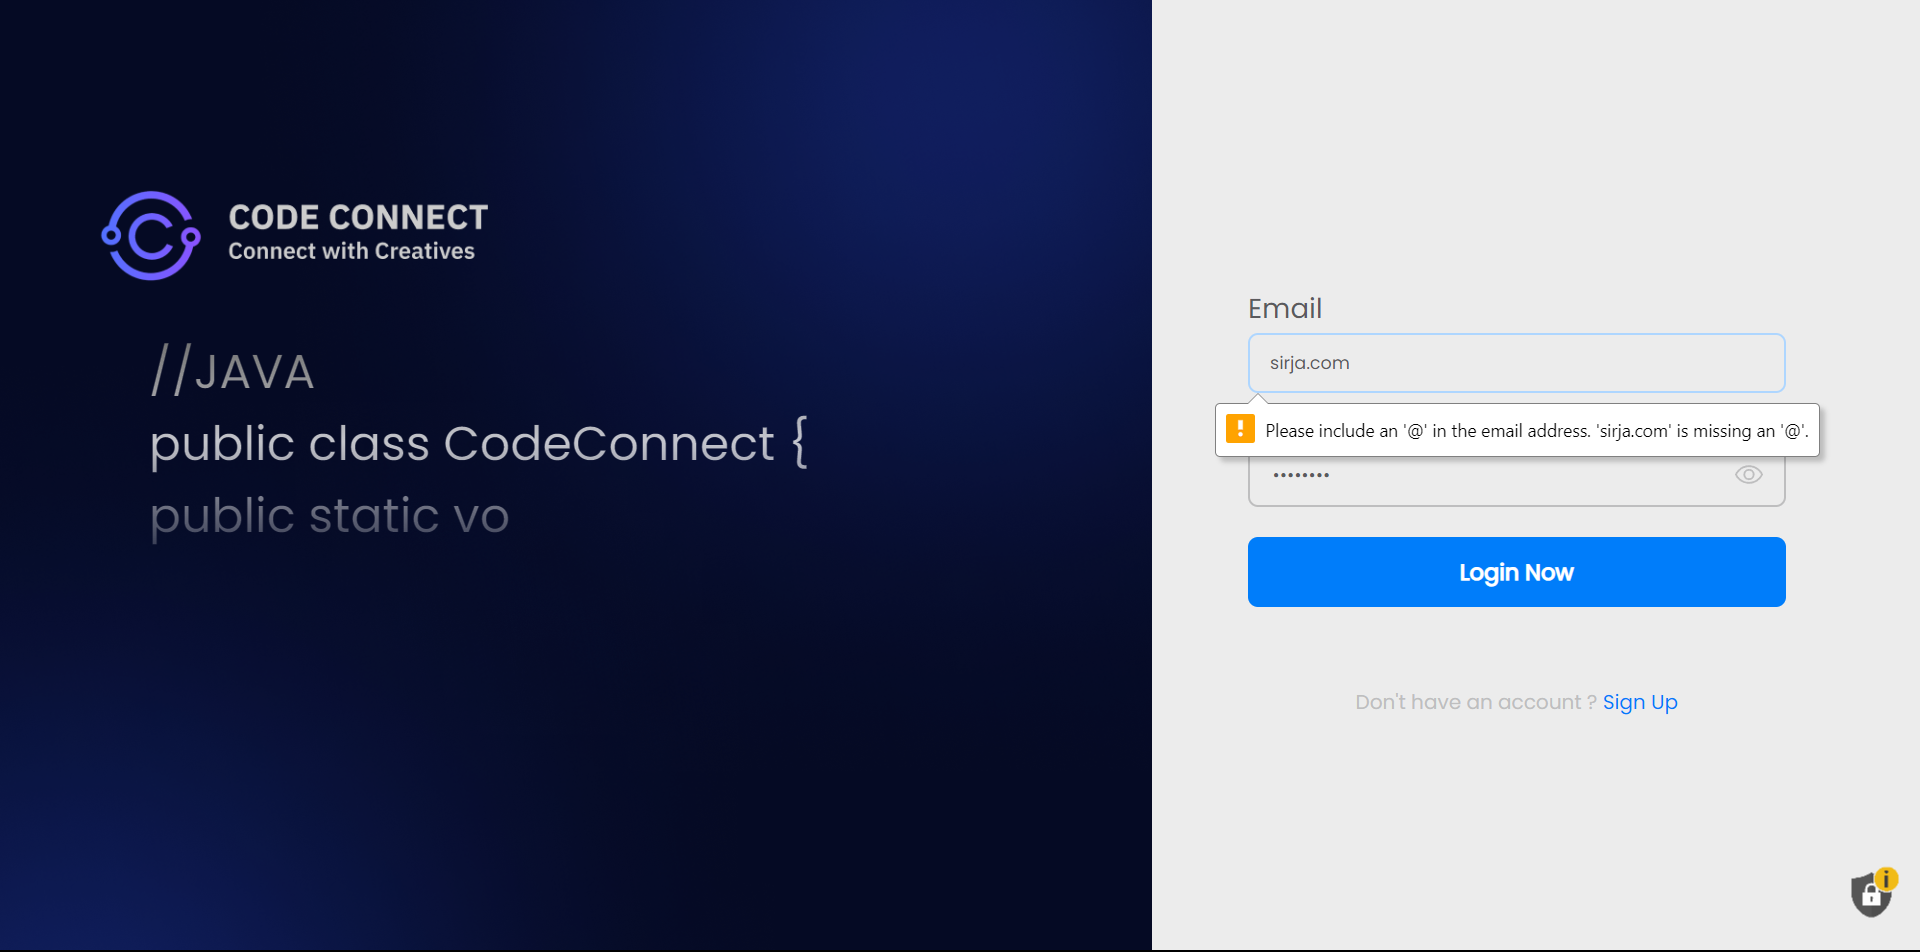
\includegraphics[width=1\textwidth]{4ImplementationAndTesting/screenshots/email-err-signin.png}
%     \caption{Incorrect email Format}
%     \label{fig: Incorrect email Format}

% \end{figure}
% \begin{figure}[ht]
%     \centering
%     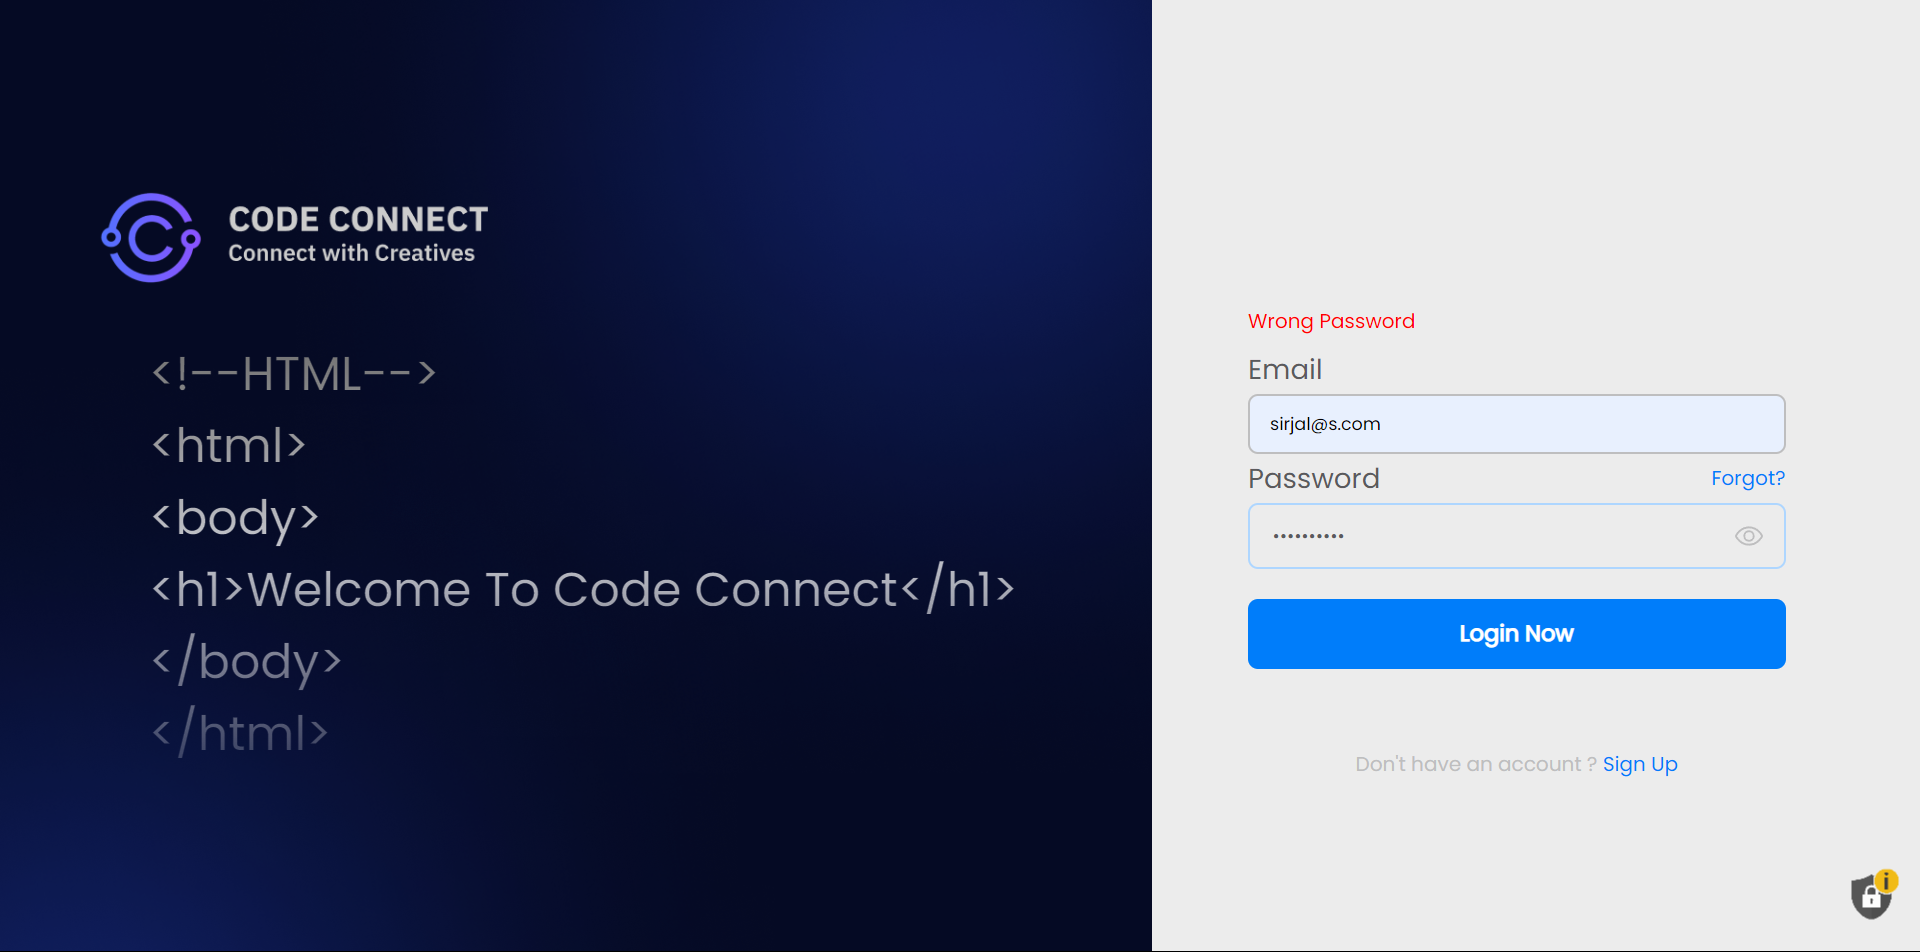
\includegraphics[width=1\textwidth]{4ImplementationAndTesting/screenshots/signin-pass-err.png}
%     \caption{Incorrect Password}
%     \label{fig: Incorrect Password}
% \end{figure}
% \begin{figure}[ht]
%     \centering
%     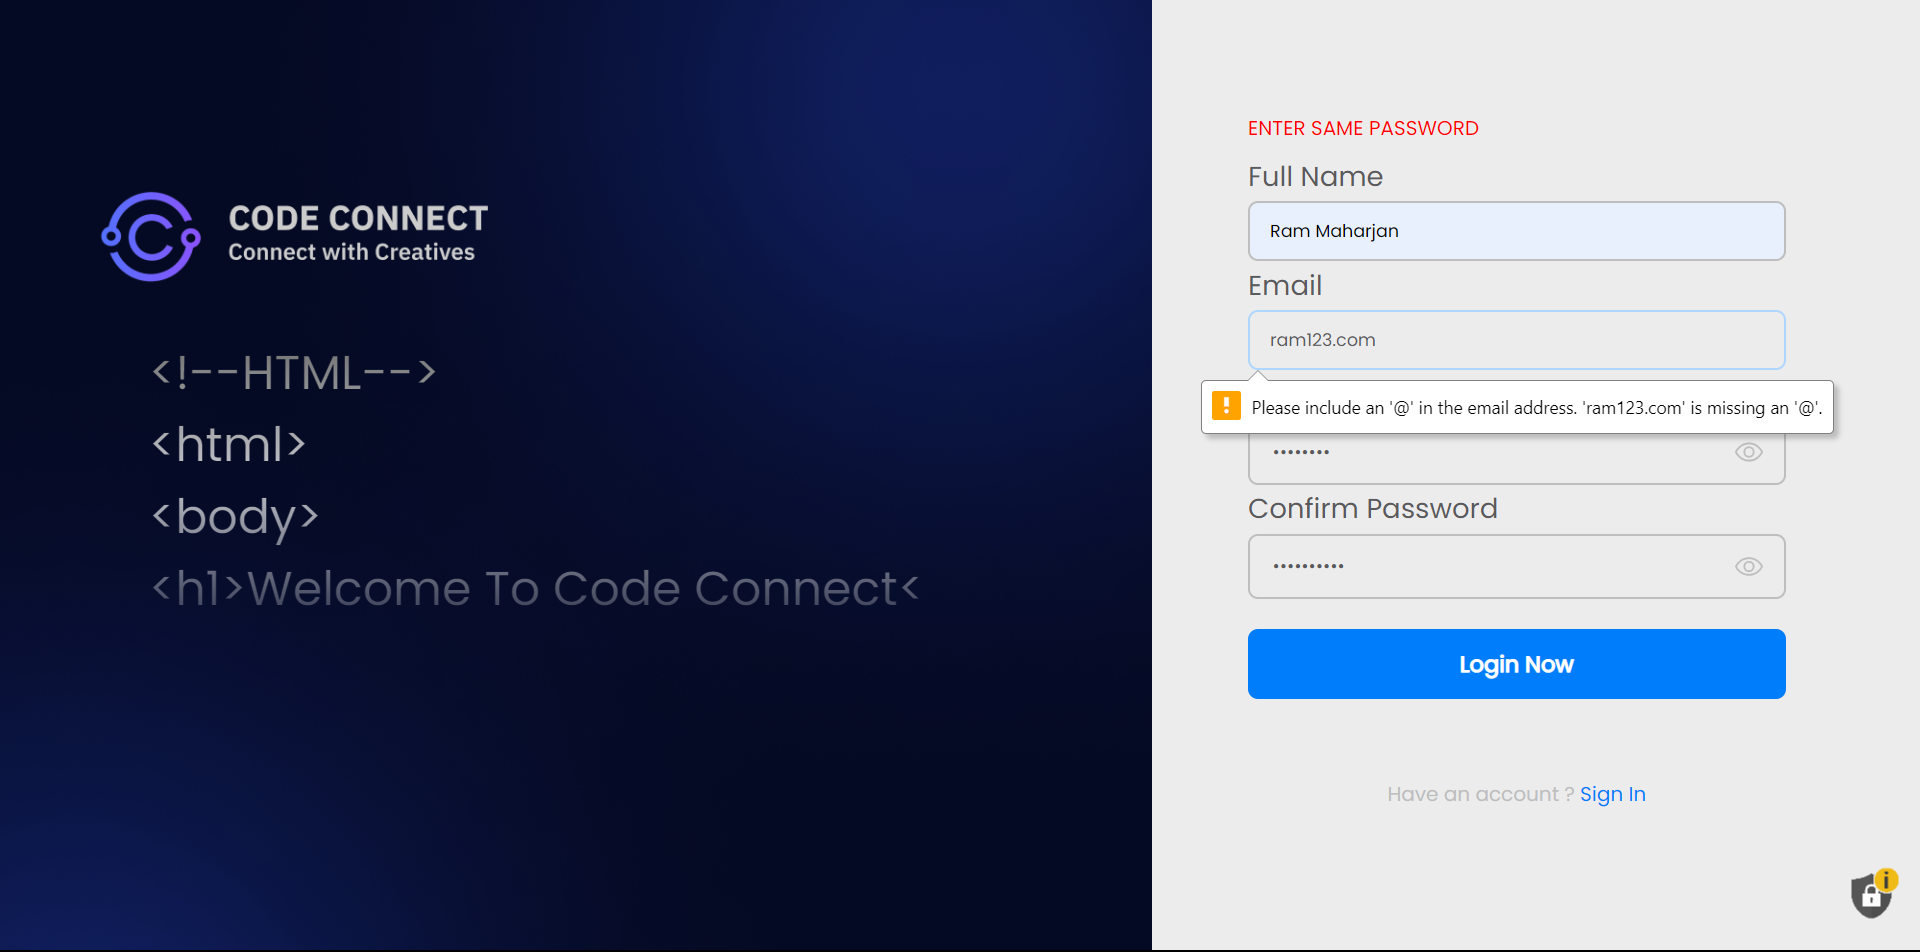
\includegraphics[width=1\textwidth]{4ImplementationAndTesting/screenshots/signup-same-pass.png}
%     \caption{Incorrect email Format In SignUp}
%     \label{fig: Incorrect email Format In SignUp}
% \end{figure}
% \begin{figure}[ht]
%     \centering
%     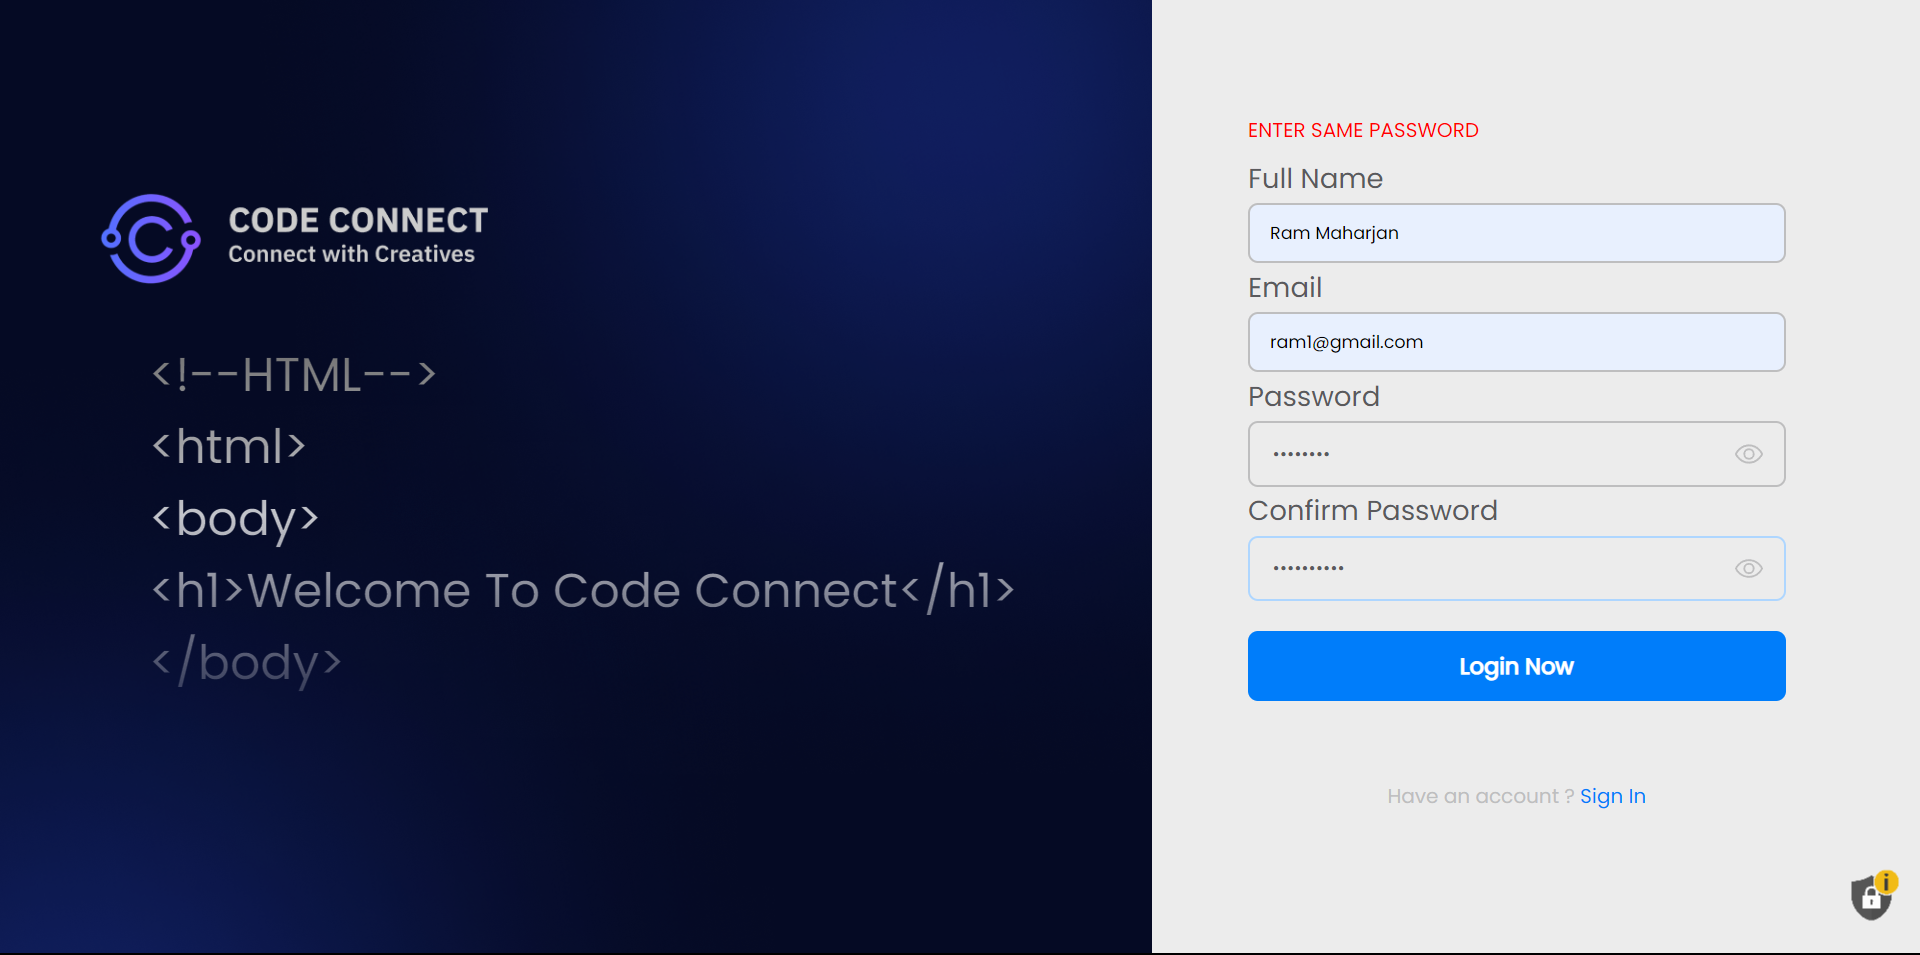
\includegraphics[width=1\textwidth]{4ImplementationAndTesting/screenshots/signup-pass-err.png}
%     \caption{Incorrect Confirm Password}
%     \label{fig: Incorrect Confirm Password}
% \end{figure}
% \begin{figure}[ht]
%     \centering
%     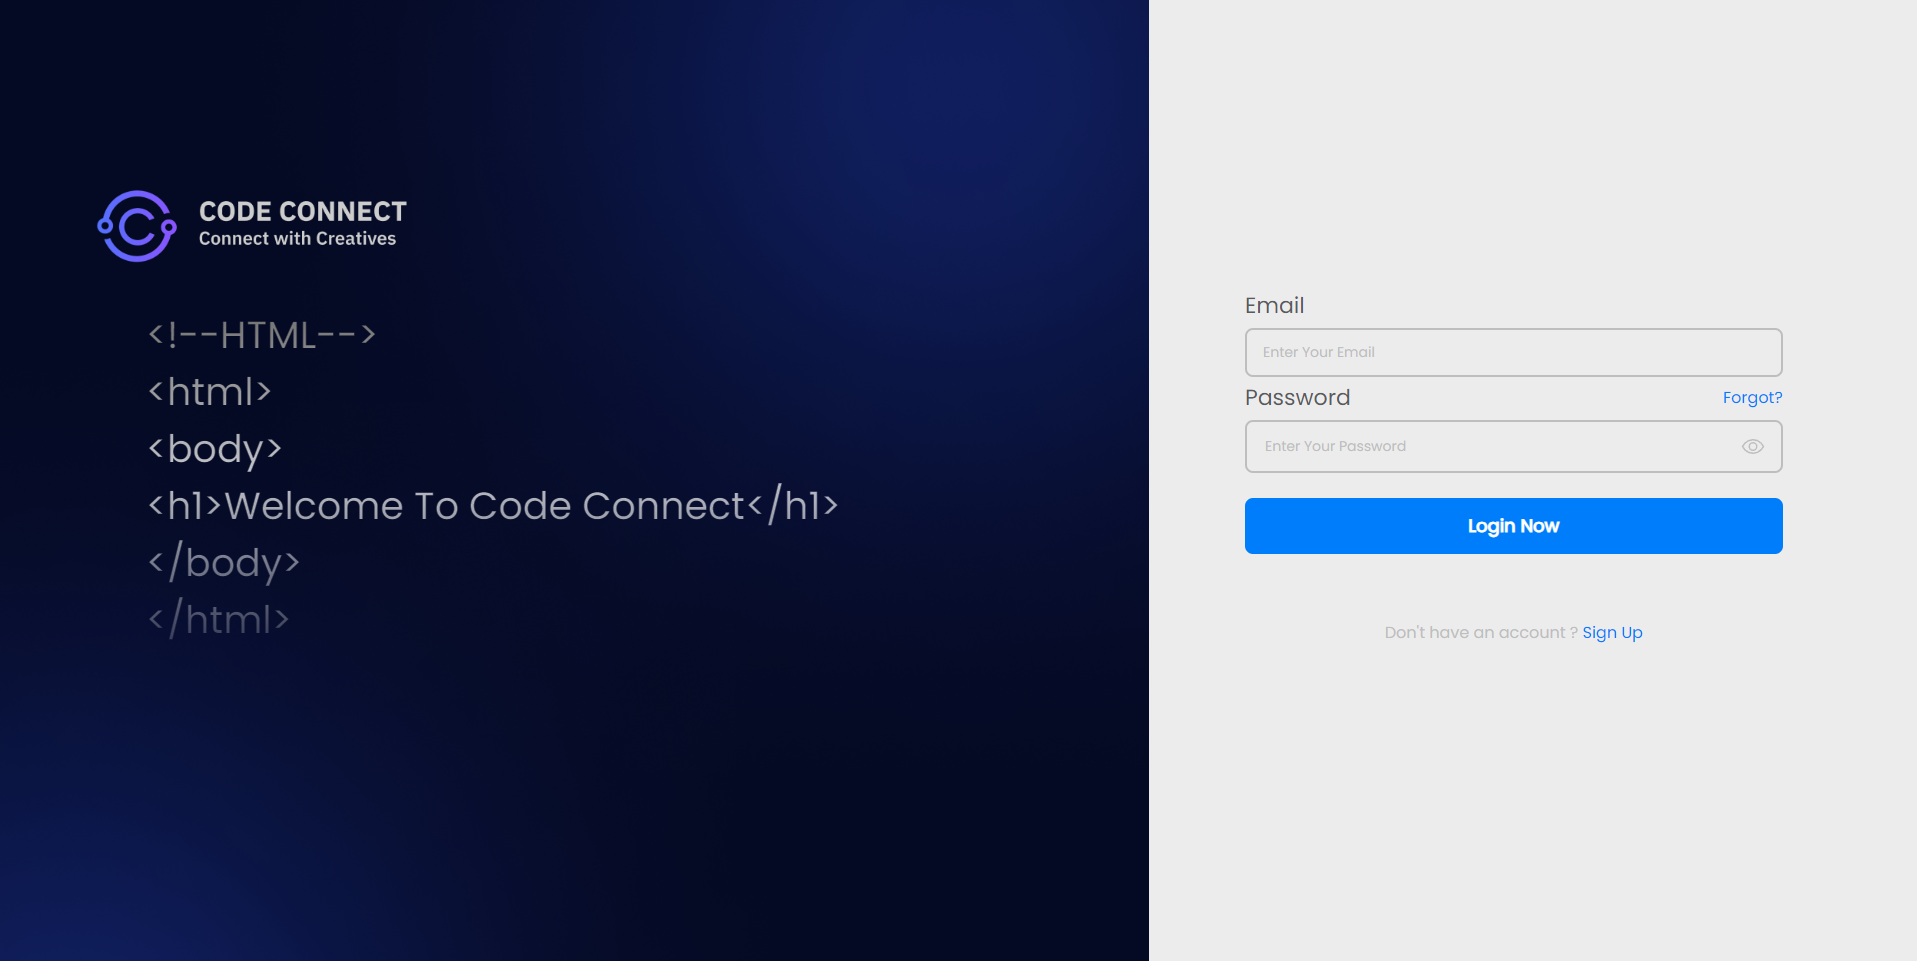
\includegraphics[width=1\textwidth]{ui_diagrams/desktop_login.png}
%     \caption{Correct SignUp Info Output}
%     \label{fig: Correct SignUp Info Output}
% \end{figure}
% \begin{figure}[ht]
%     \centering
%     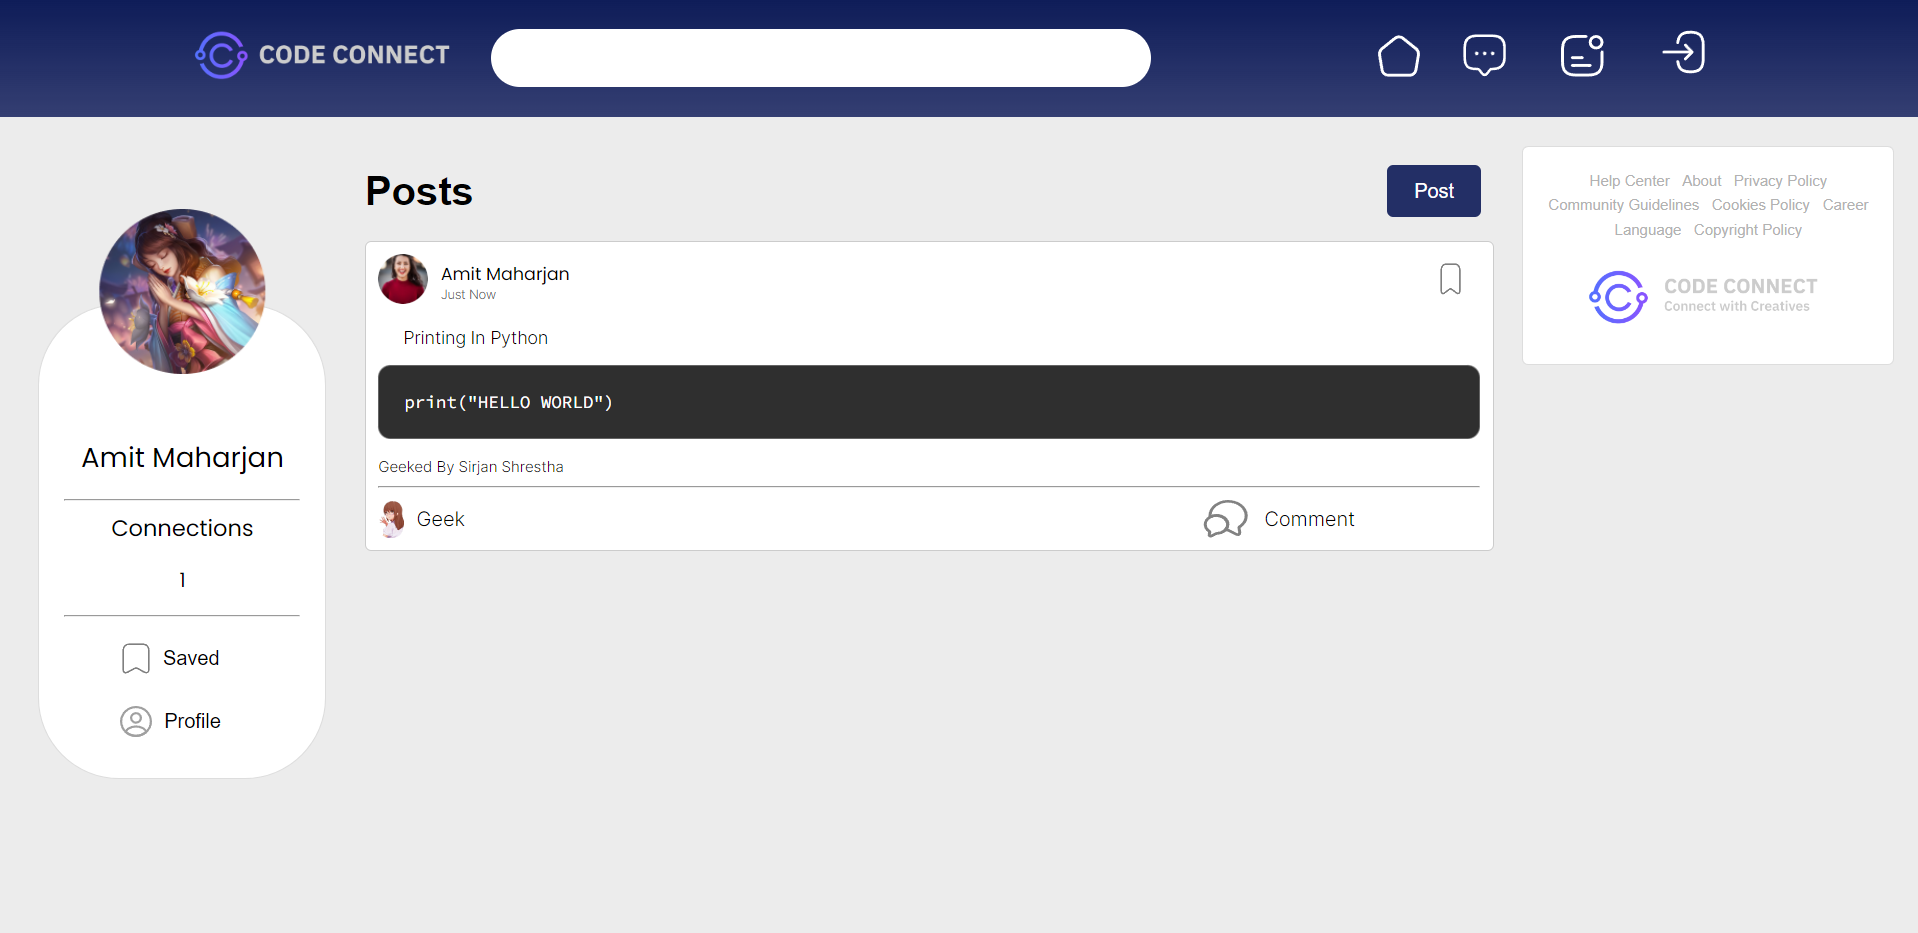
\includegraphics[width=1\textwidth]{ui_diagrams/desktop_homepage.png}
%     \caption{Correct Login Info Output}
%     \label{fig: Correct Login Info Output}
% \end{figure}

